\documentclass[11pt,aspectratio=169]{beamer}
\usepackage[T1]{fontenc}
\usepackage[utf8]{inputenc}
\usepackage[polish]{babel}
\usepackage{newtxtext,newtxmath}
\renewcommand{\familydefault}{\sfdefault}
\usepackage{microtype}
\usepackage{booktabs,tabularx}
\usefonttheme{professionalfonts}

\definecolor{ink}{HTML}{172E3D}
\definecolor{accent}{HTML}{148A76}
\definecolor{muted}{HTML}{546B7B}
\setbeamercolor{normal text}{fg=ink,bg=white}
\setbeamercolor{frametitle}{fg=ink,bg=white}
\setbeamercolor{structure}{fg=accent}
\setbeamercolor{footline}{fg=muted,bg=white}
\setbeamerfont{frametitle}{family=\sffamily,size=\Large,series=\bfseries}
\setbeamerfont{footline}{size=\tiny}
\setbeamertemplate{navigation symbols}{}
\setbeamertemplate{headline}{}
\setbeamersize{text margin left=8mm,text margin right=8mm}
\setbeamertemplate{frametitle}{%
  \nointerlineskip
  \begin{beamercolorbox}[wd=\textwidth,sep=0pt]{frametitle}%
    \usebeamerfont{frametitle}%
    \vskip3mm
    \strut\insertframetitle\strut\par
    \vskip2mm
    {\color{accent}\hrule height 0.4pt}%
    \vskip2mm
  \end{beamercolorbox}%
}
\setbeamertemplate{footline}{%
  \leavevmode\hbox{%
    \begin{beamercolorbox}[wd=0.8\paperwidth,ht=3mm,dp=2mm,leftskip=8mm]{footline}%
      PONG / Zespół 1
    \end{beamercolorbox}%
    \begin{beamercolorbox}[wd=0.2\paperwidth,ht=3mm,dp=2mm,rightskip=8mm plus 1fil]{footline}%
      \hfill\insertframenumber\,/\,\inserttotalframenumber
    \end{beamercolorbox}%
  }%
}
\setlength{\parskip}{5pt}
\graphicspath{{../wyniki/}}
\title{PONG - przeciwnik uczący się grać}
\author{Artur Zamorowski, Kacper Wojtowicz, Rafał Wybraniec}
\hypersetup{
  pdftitle={PONG - przeciwnik uczący się grać},
  pdfauthor={Artur Zamorowski, Kacper Wojtowicz, Rafał Wybraniec},
  pdflang={pl-PL}
}


\begin{document}

\begin{frame}[t]{Pong. Przeciwnik uczący się grać}
  \begingroup\large Cztery modele tablicowego Q-learningu\par\endgroup
  \vspace{2mm}
  \begin{columns}[T,onlytextwidth]
    \begin{column}{0.54\textwidth}
      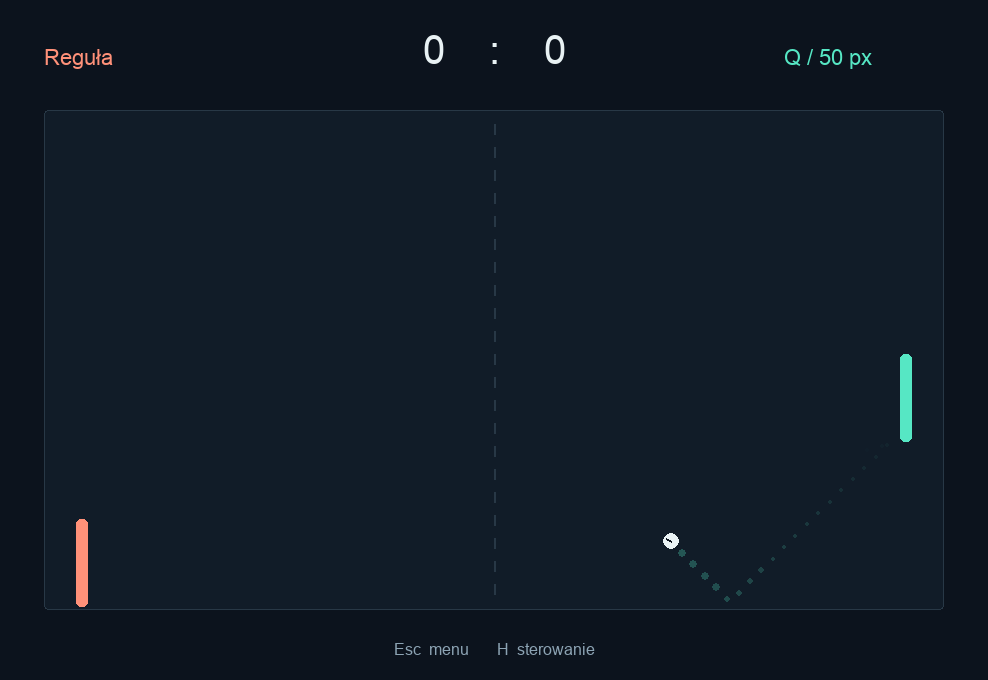
\includegraphics[width=\linewidth,height=46mm,keepaspectratio]{gra.png}
    \end{column}
    \begin{column}{0.39\textwidth}
      \vspace{3mm}
      Artur Zamorowski\\
      Kacper Wojtowicz\\
      Rafał Wybraniec

      \vspace{8mm}
      Projekt 1\\
      Poniedziałek 8:00
    \end{column}
  \end{columns}
\end{frame}

\begin{frame}[t]{Gra i fizyka}
  Agent steruje prawą paletką. Wybiera ruch w górę, postój albo ruch w dół.
  Dostaje pozycję i prędkość piłki oraz własnej paletki.

  \vspace{4mm}
  Fizyka: \textbf{120~Hz}. Decyzje obu paletek: \textbf{30~Hz}.
  Miejsce trafienia i ruch paletki zmieniają kąt odbicia oraz rotację piłki.

  \vspace{4mm}
  Trening bez grafiki i gra korzystają z tej samej symulacji.
  Cztery moduły: uruchamianie, fizyka, agenci i interfejs.
  Parametry są w jednym pliku YAML.
\end{frame}

\begin{frame}[t]{Tablica Q}
  Stan: pozycje piłki i paletki w siatce, znak $v_x$,
  kategorie $v_y$ piłki i prędkości paletki.
  Każdy stan ma trzy wartości Q, po jednej dla każdej akcji.

  \[
    Q(s,a)\leftarrow Q(s,a)+\alpha\left[r+\gamma\max_{a'}Q(s',a')-Q(s,a)\right].
  \]

  Nagroda: $+1$ za punkt, $-1$ za stratę i $+0{,}2$ za odbicie.
  $\gamma=0{,}98$.

  \vspace{3mm}
  Epsilon maleje od 0,9 do 0,05. W ocenie wynosi zero.
  Każdy trening zaczyna od zerowej tablicy.
\end{frame}

\begin{frame}[t]{Porównanie parametrów i pokaz}
  Siatki \textbf{50 i 100~px}. Alfa \textbf{0,12 i 0,35}.
  Cztery treningi po \textbf{50\,000 epizodów}.

  \vspace{4mm}
  Ocena końcowa: 450 wspólnych serwisów na politykę.
  Przeciwnik podąża za bieżącą wysokością piłki.
  Limit punktu w ocenie: 20~s.

  \vspace{4mm}
  \texttt{python kod/main.py play}

  W \texttt{konfiguracja.yaml} ustaw \texttt{demo: true}.
  W/S: ruch. Spacja: pauza. D: pokaz. R: nowy mecz.
\end{frame}

\begin{frame}[t]{Wyniki oceny końcowej}
  \begin{tabularx}{\linewidth}{@{}Xrr@{}}
    \toprule
    Polityka & Wygrane & Średnia liczba odbić \\
    \midrule
    50~px, $\alpha=0{,}12$ & 66 (14,7\%) & 6,45 \\
    50~px, $\alpha=0{,}35$ & 18 (4,0\%) & 3,97 \\
    100~px, $\alpha=0{,}12$ & 15 (3,3\%) & 3,61 \\
    100~px, $\alpha=0{,}35$ & 6 (1,3\%) & 2,49 \\
    Reguła & 77 (17,1\%) & 12,43 \\
    \bottomrule
  \end{tabularx}

  \vspace{4mm}
  Najlepszy model Q: 50~px, alfa 0,12.
  Reguła uzyskała wyższy odsetek wygranych i dłuższe wymiany
  od każdego z czterech modeli.
\end{frame}

\begin{frame}[t]{Podział pracy i dalsze kroki}
  \begin{tabularx}{\linewidth}{@{}lX@{}}
    Artur Zamorowski & Budowa i trenowanie modelu. \\
    Kacper Wojtowicz & Gra, interfejs i prezentacja. \\
    Rafał Wybraniec & Sprawozdanie, dokumentacja i dobór parametrów. \\
  \end{tabularx}

  \vspace{7mm}
  Wyniki pochodzą z jednego ziarna treningu na wariant.
  Kolejny eksperyment: więcej ziaren uczenia i większy budżet
  dla dokładniejszej siatki.
\end{frame}

\end{document}
